\documentclass[a4paper,12pt]{article} 
%\usepackage{coloremo/coloremoji}
\usepackage[english,russian]{babel}
% \usepackage{xecyr}
\usepackage{enumitem}
\usepackage{longtable}
\usepackage{ifthen}
\usepackage{mathtext}
\usepackage{graphicx}
\usepackage{listings}
\usepackage{afterpage}
\usepackage{url}
\usepackage{fancyvrb}
\usepackage{color}
\usepackage{hyperref}
\usepackage{booktabs}
% \usepackage[citestyle=alphabetic,bibstyle=authortitle]{biblatex}
% \setmainfont{Calibri}
\title{Udaff — русский пиктографический Python. От элементарных алгоритмов до гомоморфного шифрования}
\date{2020 \\ Январь}
\author{Стас Фомин, stas-fomin@yandex.ru} 

\providecommand{\tightlist}{%
     \setlength{\itemsep}{0pt}\setlength{\parskip}{0pt}} 

\begin{document}
\maketitle
\begin{abstract}
    Автор часто встречал изобретения «специальных языков для обучения программированию», кривых и убогих, с жалкой инфраструктурой и поддержкой, отрезанных от мирового мейнстрима программирования и обучения, при этом навязываемых в школах и ВУЗах. Иногда необходимость таковых обосновывается требованиями «русскоязычности» ключевых слов. 

    Предлагается шире использовать Python — язык, годный от обучения дошкольников до глубокого профессионального использования во многих областях. А если кому-то нужна именно русскоязычность ключевых слов — туда ее можно добавить, что и проделал автор, не нарушив совместимости. Кроме русскоязычности добавлены и пиктограммы, эмоджи — возможно это тоже поможет в обучении начинающим, а возможно это пригодится и взрослым — для компактизации описаний нетривиальных алгоритмов.

    Работа выполнена при поддержке гранта РФФИ 19-01-00702А.
\end{abstract}

\section{Проблема}

В русскоязычном пространстве наблюдается странный эффект изобретения
«русскоязычных» языков программирования, и попыток навязать их
обучающимся в Школе и ВУЗе.  

См. например Кумир \cite{kumir}, SLang \cite{slang}
(не путать с еще одной самоделкой --- СЛанг \cite{slang2})\ldots{} множество их.
  
С одной стороны, вроде как основания есть --- из-за специфики высшего
образования в РФ (бесплатное образование, оплачивается ВУЗам МинОбром
подушевым образом, отчислять невыгодно, и даже запрещено \cite{fire-restricted}), 
в ВУЗы на околопрограммиские специальности попадает множество немотивированных и
функционально необразованных кадров, не способных понимать даже текст с
десятком ключевых слов на английском. С другой стороны, возможно успех
таких платформ типа 1C именно этим и обусловлен, да и есть немало
энтузиастов, которые
считают, что русификация ЯП --- полезна \cite{russification-good}, и
учить на русифицированных
языках эффективно \cite{russification-effective}.

Однако проблема всех этих самоделок в том, что язык --- это не только
синтаксис грамматики в BNF на полстраницы, а это инфраструктура:

\begin{itemize}
\tightlist
\item
  Редакторы, IDE, поддерживающие 100500 удобных фич, не говоря уже о
  обязательной «построчной» отладке.

  \begin{itemize}
  \tightlist
  \item
    Разработчики «Русских ЯП» пытаются делать некие подобия IDE, благо
    сейчас это можно слепить из каких-нибудь готовых компонентов (модуль
    текстового редактора с подсветкой, MDI интерфейс с менюшками) --- но
    все что получается, это скажем прямо, уровень 90х, и сравнивая это с
    бесплатным и open-source «швейцарским ножем» Visual Studio Code, (не
    говоря уже о коммерческих IDE) хочеться только плакать от жалости.
  \end{itemize}
\item
  Инфраструктура пакетов (сами библиотеки, пакетные менеджеры), 100500
  пакетов для решения всего скучного и типового, не говоря уже о
  нетривиальных платформах (быстрый вход в разработку игр,
  математические методы и AI и т.п.)
\item
  Правильные концепции и парадигмы языка, проверенные десятилетиями
  обкатки на миллионном комьюнити профессионалов.
\item
  Возможность получения профессиональных НАВЫКОВ, вшитых на уровень
  костного мозга, которых можно применить в профессиональной разработке
  для решения реальных проектов. Чтобы стартовав с элементарных
  алгоритмов и простых поделий, можно было эволюционировать в
  профессионала.
\end{itemize}

Но если «показать что-то про программирование на русском», на уровне
«операторы-ветвление-цикл-функция-рекурсия» для совершенно левых людей
(которым максимум в 1C в жизни придется что-то подправить) ---
допустимо, то совращать «девственно» чистых школьников кривыми
поделиями, отрубая им прямой выход к реальной разработке и отбивая
желание программировать («пробовал ваше программирование на К\ldots{} »
--- ничего не работает, тормозит, криво, неудобно, долбайтесь сами), как
минимум неэтично, хотя к сожалению, уголовно ненаказуемо.

Кстати, иногда изобретают «еще одну платформу для обучения» даже не для
русификации языка, а для, скажем так, «реанимации стюардессы», типа
паскаля, но проблемы остаются те
же --- какое-то свое подмножество языка, унылые среды разработки, все
сбоку от майнстрима и сообщества \cite{pascal-sucks}.

Возникает дилемма --- как бы убить двух зайцев --- пользуясь одной
платформой дать возможность неодаренным и негодным
студентам и школьникам \cite{students-sucks} «попробовать программирование», а продвинутым,
тут же, в том же классе, на том же софте, дать возможность уйти в отрыв
и стать настоящими профессионалами.

\section{Решение}

Итак, уже есть Python, идеальный язык для обучения, рожденный как язык
для обучения, десятилетиями использующийся от везде --- от уровня
младших школьников, до профессионалов, как в программировании, так и в
куче научных областей --- будь то астрономия, биоинформатика,
статистика\ldots{} везде.

Знание его полезно, если не сказать необходимо, даже тем, кто не
программист, если деятельность хоть как-то интеллектуальна (да, даже
если экономист-юрист уровня выше чем «за рубль покупаем, за три продаем,
на эти два процента и живем»).

К нему есть куча IDE, включая прекрасную поддержку даже в бесплатном и
свободном Visual Studio Code (не нужно
изобретать страшные велосипеды \cite{ide-python}), есть
100500 пакетов, платформы для написания всего --- игр, десктоп и
вебприложений, даже мобильной и IOT разработки\ldots{} Впрочем, все это
банально и очевидно.
 
Наша идея \cite{python-udaff} --- добавить еще «маленькую лесенку» снизу, разрешив писать
ключевые слова и базовые функции на русском, для тех, кто вот только
стартует, не потеряв никаких возможностей Python.

Для этого можно воспользоваться идеей «пользовательских кодировок»,
перекодирующих файл с программным кодом при открытии. В результате,
несколько десятков ключевых слов Python приводятся к каноническому
английскому виду, их понимает и язык, и отладчики и т.п. А обучающийся
имеет полную возможность, по мере изучения, постепенно заменить «русские
аналоги» их оригинальными ключевыми словами, и с улыбкой (но без
ненависти) забыть свои самые первые программы.

\begin{figure}
\centering
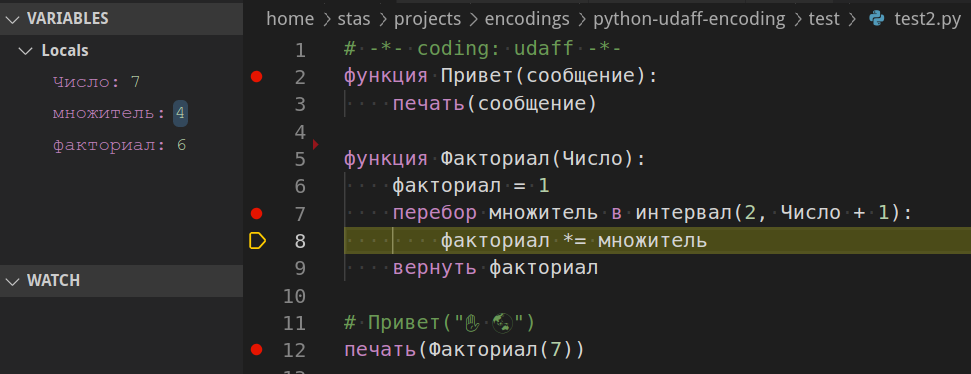
\includegraphics[width=\textwidth]{pictures/factorial.png.eps}
\caption{Пример отладки «факториала}
\end{figure}

\begin{longtable}[]{@{}ll@{}}
\toprule
Английский & Русский\tabularnewline
\midrule
\endhead
and & и\tabularnewline
as & как\tabularnewline
assert & проверить\tabularnewline
break & прервать\tabularnewline
class & класс\tabularnewline
continue & продолжить\tabularnewline
def & функция\tabularnewline
del & удалить\tabularnewline
elif & ежели\tabularnewline
else & иначе\tabularnewline
except & случись\tabularnewline
exec & выполни\tabularnewline
finally & наконец\tabularnewline
for & перебор\tabularnewline
from & из\tabularnewline
global & глобальное\tabularnewline
if & если\tabularnewline
import & подключить\tabularnewline
in & в\tabularnewline
is & суть\tabularnewline
lambda & лямбда\tabularnewline
not & не\tabularnewline
or & или\tabularnewline
pass & ничего\tabularnewline
print & печать\tabularnewline
raise & паника\tabularnewline
return & вернуть\tabularnewline
try & пробовать\tabularnewline
while & повторять\tabularnewline
with & пусть\tabularnewline
yield & вернуть\tabularnewline
range & интервал\tabularnewline
\bottomrule
\end{longtable}

Лично я (Стас Фомин), не считаю, что это необходимо. На мой взгляд лучше
таки выучить эти пару десятков ключевых слов Python на английском, и
отсеять «электорат» с уровнем IQ меньше веса.\\
Но идя путем «выбора меньшего зла» (\emph{toss a coin to\ldots{}}), я
уверен, что этот подход лучше изобретения кривых велосипедов  от
скучающих преподавателей, которые будут калечить поколения школьников
и студентов. Т.е. я был бы рад, если все это не
пригодилось при обучении, но при встрече с изобретателем очередного
«национального языка», у меня будет куда его конструктивно послать.

С другой стороны, может это пригодится где-то, где Python используется
как DSL для какой-нибудь бизнес-логики --- короткие функции, которых
должны править и вычитывать специалисты  в предметной области,
может это пригодится и там.

Более того, можно привлечь к программированию, совсем, так сказать,
правополушарных людей, и использовать вместо идентификаторов функций
и переменных значки emoji.

Если серьезно, то можно использовать и имеющуюся в юникоде «математику»,
и символы-эмотиконы, для того, чтобы компактифицировать 
реальные работающие алгоритмы, для преподавания или верификации,
особенно нетривиальных алгоритмов 
(автор пробовал описывать блокчейны и гомоморфное шифрование).

\begin{figure}
\centering
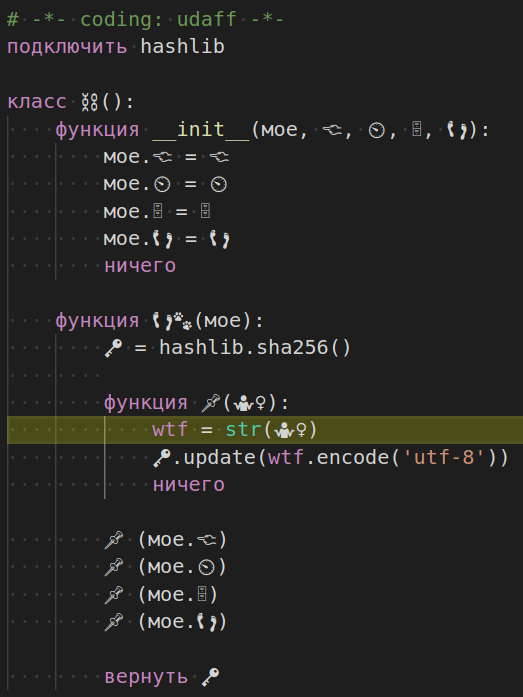
\includegraphics[width=0.7\textwidth]{pictures/blockchain.png.eps}
\caption{Часть работающего «русифицированного» блокчейна}
\end{figure}


Ну а название «udaff», отсылает к популярному времен начала Рунета
ресурсу, который прекрасно иллюстрировал идею, что буквоедство и
грамотность не так важны, как суть и контент, а иногда такое «грязное
языковое хакерство», как кстати, в предложенном решении, даже весело.
Кстати, тут несложно сделать и поддержку разных версий «падонкоффского
языга».

\begin{thebibliography}{9}
    \bibitem{kumir} Доклады о языке Кумир, \url{http://0x1.tv/Kumir}

    \bibitem{slang} «Обучающая среда по программированию на базе СПО (Валерий Лаптев, OSEDUCONF-2019)», \url{http://0x1.tv/20190127E}

    \bibitem{slang2} «Проект СЛанг — текущее состояние и перспективы (Алексей Канатов, SECR-2017)», \url{http://0x1.tv/20171021CA}

    \bibitem{fire-restricted} «Отчислять отстающих запрещено», \url{https://youtu.be/LDdgdKI20cU?t=1351}
    \bibitem{russification-good} «Русификация языка -- это отдельная большая тема, и её польза лично мне очевидна», \url{http://www.0x1.tv/20191205AD#comment-4763683278}

    \bibitem{russification-effective} «учить на русифицированных
    языках эффективно», \url{https://youtu.be/LDdgdKI20cU?t=1503}
    \bibitem{pascal-sucks} «Несколько причин забыть PascalABC.Net», \url{https://habr.com/ru/post/417229/}
    \bibitem{students-sucks} «Ваши студенты олигофрены?», \url{https://youtu.be/LDdgdKI20cU?t=1144}
    \bibitem{ide-python} «IDE для изучения Python (Николай Попов, OSEDUCONF-2015)», \url{http://0x1.tv/20150124G}
    \bibitem{python-udaff} «Udaff — русификация Питона», \url{https://github.com/belonesox/python-udaff-encoding}
\end{thebibliography}
\end{document}
